\subsubsection{Soar Panel Effect (Jacob)}

The maximum output effect of the Photo Voltaics is unknown, there is no datasheed nor model number to help find information about the effect. To find out, a small test was made, first test was with thin clouds all over the sky, second test was done a day without any clouds in front of the sun.¨The moving clods during the first test interrupted the results, and they were not reliable enough.\\

\begin{figure}[H]
\centering
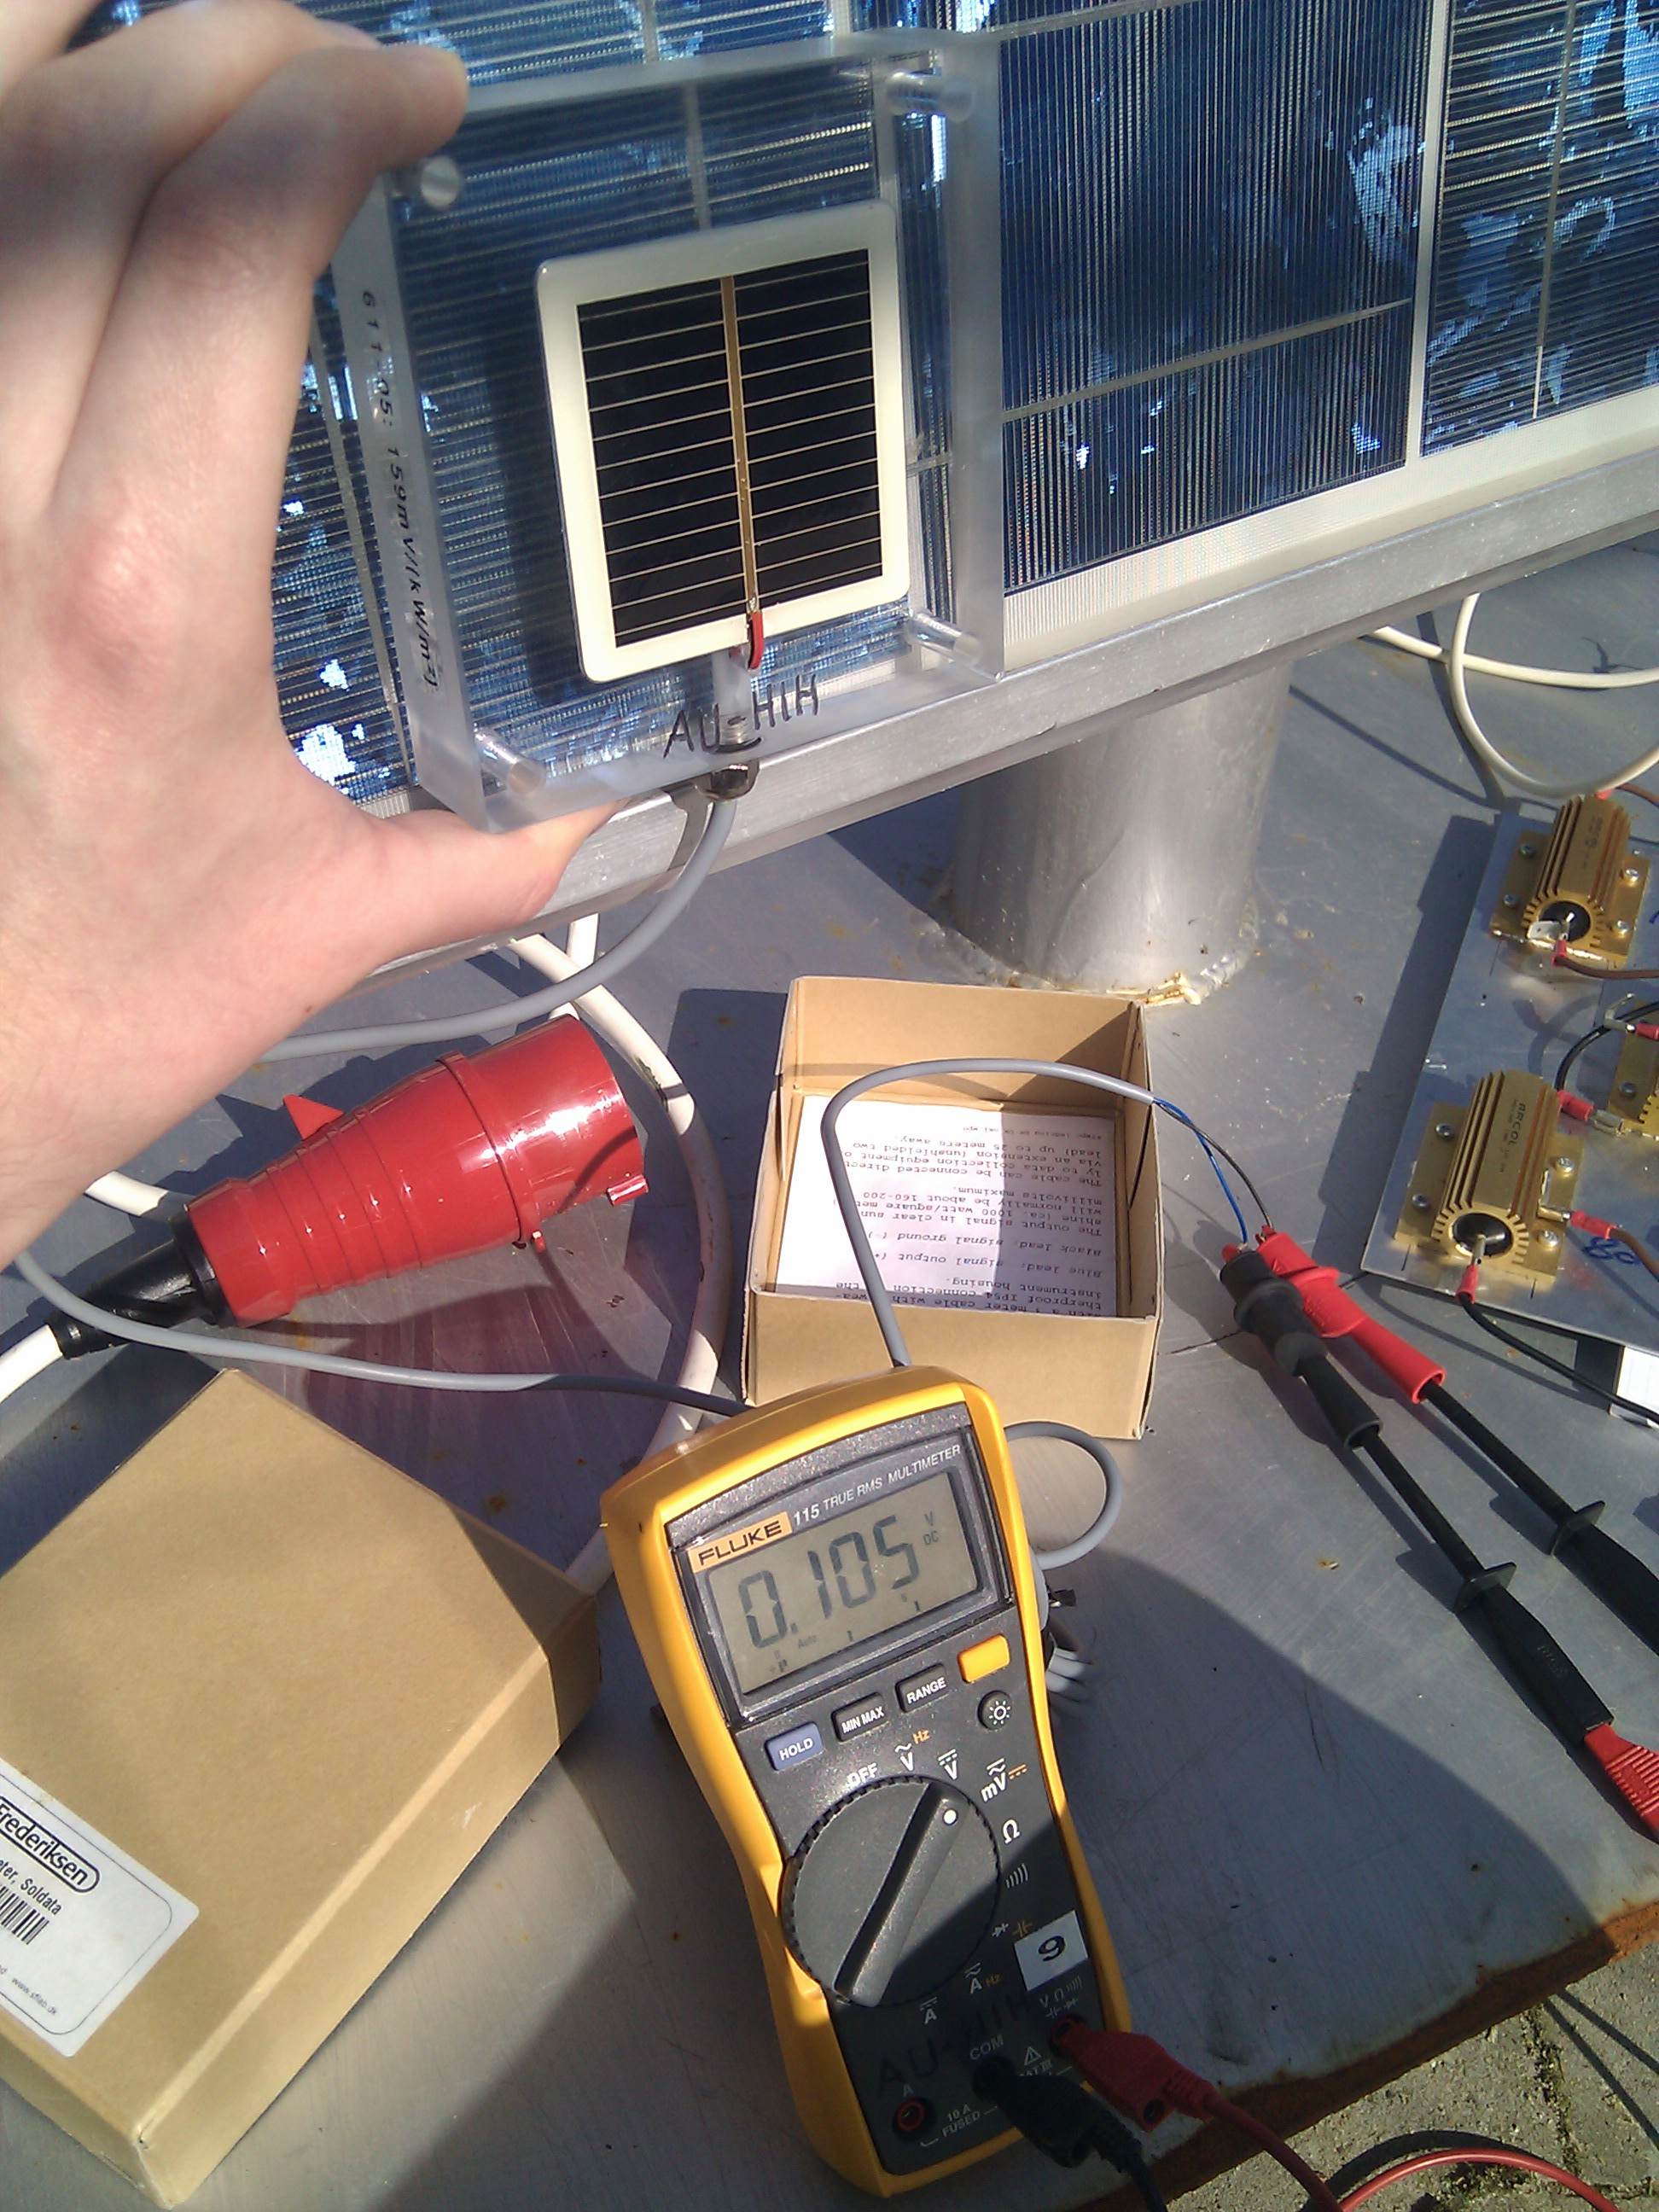
\includegraphics[width=5cm]{./img/sun_intensity}
\caption{Measuring of sun intensity}
\label{fig:sun_intensity}
\end{figure}

To find out how intense the sunlight was, a pyranometer was used. It was placed at the surface of the Photo voltaics, to measure at the same angle as the panel itself. This is shown at Figure \ref{fig:sun_intensity}. A multimeter was connected to the output, which measured 134mV. The pyranometer is calibrated to have a output of 159mV when the intensity equals $1000W/m^2$.\\
$134mV/(0.159mV/W)=842W/m^2$

\begin{figure}[H]
\centering
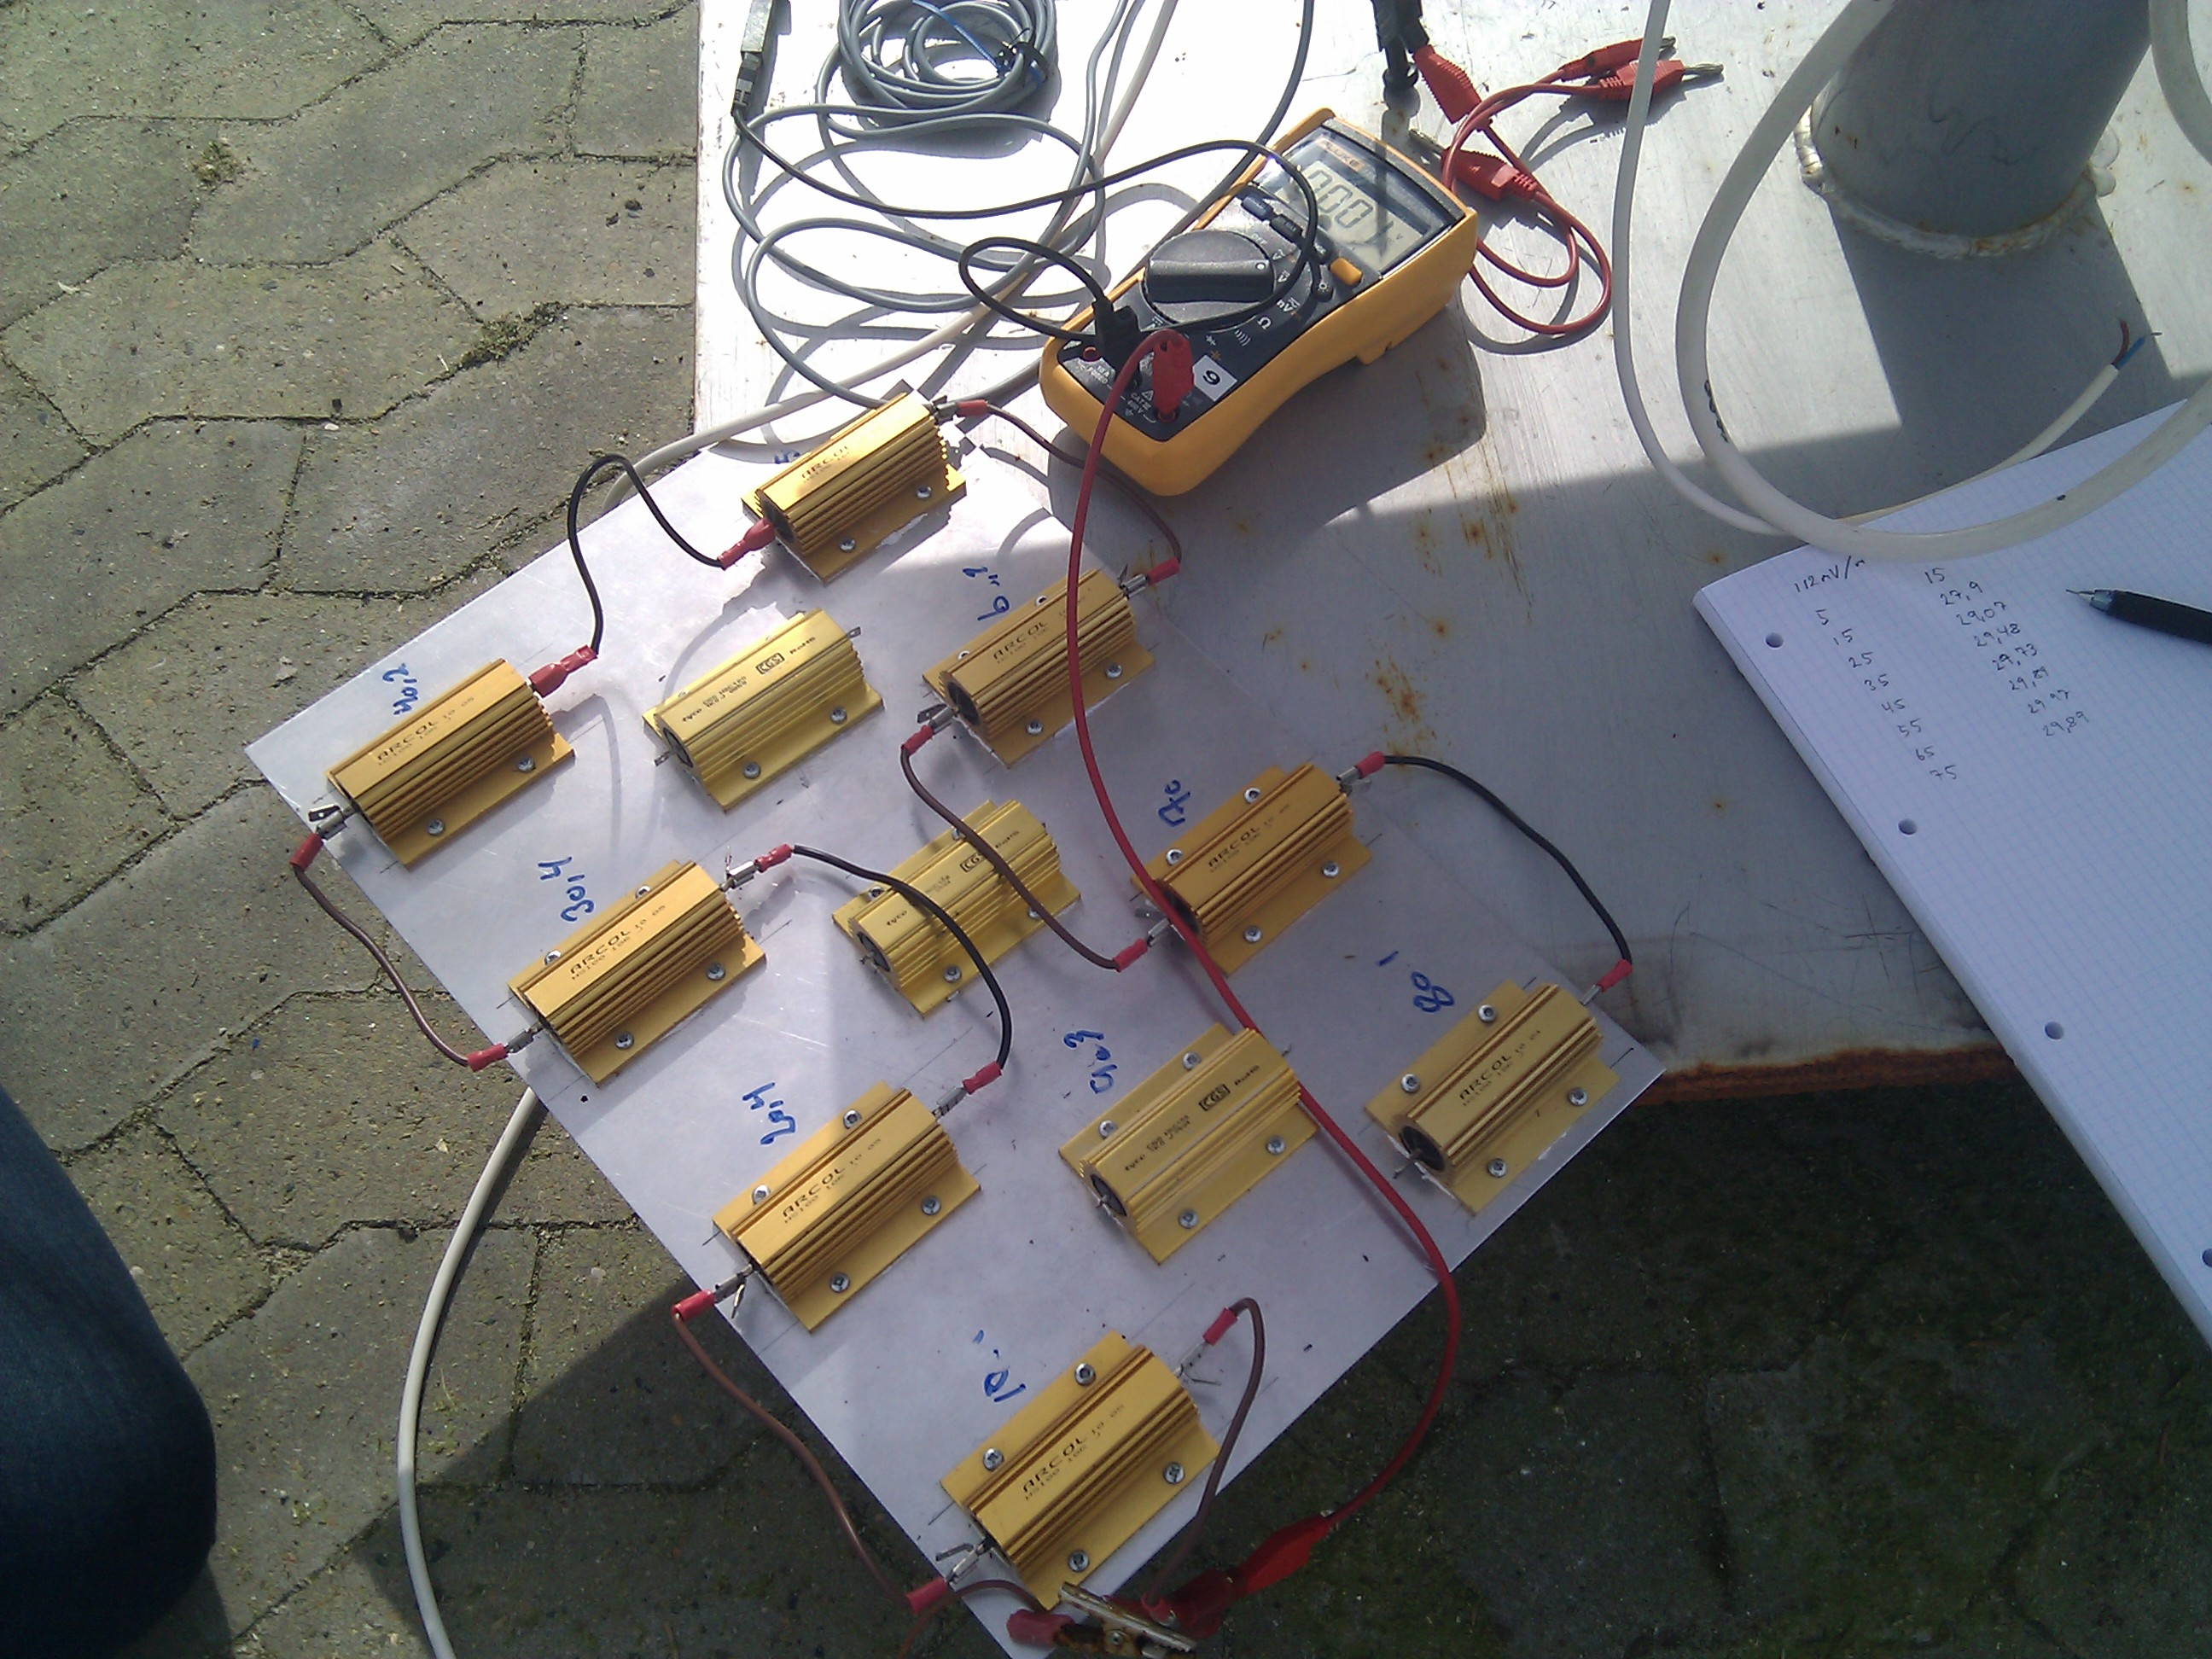
\includegraphics[width=6cm]{./img/IMG_20120326_140141}
\caption{Several resistors, to measure the effect of the Photo Voltaics}
\label{fig:IMG_20120326_140141}
\end{figure}


Now the output of the Photo Voltaic was measured. Only the output voltage was measured. It was measured across different resisstances, from 5ohms upto 125ohm, in steps of 5ohm. Then the current could be calculated from ohms law, and figures \ref{fig:Voltage_VS_Current-PV_effect} and \ref{fig:Voltage_VS_Power-PV_effect} shows the relation between load and power. \\


\begin{figure}[H]
\centering
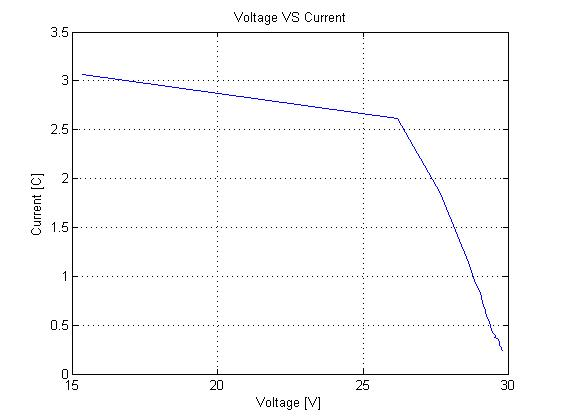
\includegraphics[width=8cm]{./img/Voltage_VS_Current-PV_effect}
\caption{Voltage VS Current - Photo Voltaics Effect}
\label{fig:Voltage_VS_Current-PV_effect}
\end{figure}

\begin{figure}[H]
\centering
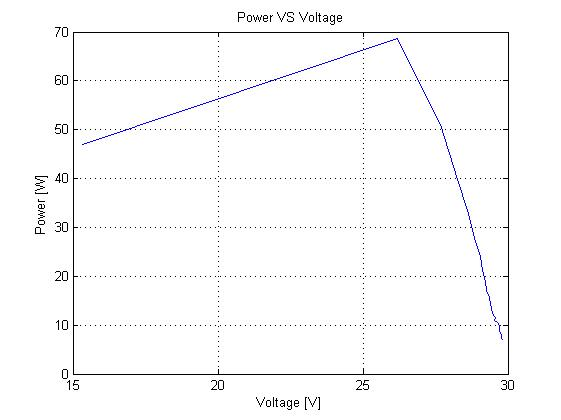
\includegraphics[width=8cm]{./img/Voltage_VS_Power-PV_effect}
\caption{Voltage VS Power - Photo Voltaics Effect}
\label{fig:Voltage_VS_Power-PV_effect}
\end{figure}

Its fund that the highest output effect is at almost 70watts. We also see that the Photo Voltaics has to be installed with the correct load, to give the highest power output. \\
This test was done on a sunny day, but not the MOST sunny day of all time. It is still unknown what the highest power output of the panel is, and it is hard to find out. \\

Other information about the panel may help, namely the open circuit voltage, measured at the output of the photo voltaics, without any load. The output was measured to 30.4V. \\
A lot of datasheets was inspected, in order to find matching photo voltaics, with the same characteristics of minimum 70W and a open circuit voltage of 30V. This voltage will not increase if the sun intensity increases, only the amperes will. This is the maximum voltage output, so that has to be fulfilled in the datasheet. The one matching the best, was from gernam solar power; GSP-P50-185. \hilight{\textbf{[DATASHEET]}} \\
The important properties that was compared:\\

\begin{tabular}{|l|l|l|}
\hline  & Data & Datasheet \\ 
\hline Open-circuit voltage Voc & 30.4V & 30.65V \\ 
\hline Rated voltage Vmpp & 70W & 185Wp \\ 
\hline 
\end{tabular} 

The open circuit voltage is very close to the target, but the watt-peak is not that close. The Watt-peak is measured in labs,m by applying $1000W/m^2$ to the Photovoltaics panel, and then measure the output across different resistances. Fortunately such a strong light is not available for us to use, but in the test made, the power was at $842W/m^2$. Another error is the "big" step in resistance. The rated voltage (Vmpp) of the target panel is at 25.05V. In the test made, a voltage was measured to 15.32V and 26.19V at 5 and 10 ohm resistance respectively. A resistance of lets say 8ohm may have lifted the watt-peak a bit. With these twop ewrrors in mid, the lack of $watt/m^2$ and the unprecise resistance may have decreased the performance of the panel. In order to the project work to contunie, this datasheet will be used, to find the highest voltage and current output of the photovoltaics. \\

Another important thing about these results, is that we doint need any galvanic isolation in the system. 30V and 8A is not enough to damage and/or disturb the PCBs, more than the problems it provokes can be solved in other, more cheaper and easier ways. 







\subsubsection{Design circuit for Log Module (Jacob)}
\paragraph{Requirements to fulfil}\mbox{}\\
FR.1.d\\
NR.1.a\\
None of the requirements will be completely fulfilled in this timebox, but during this period both should be kept in mind. 
\paragraph{Theory}\mbox{}\\

\begin{landscape}
\begin{figure}[H]
\centering
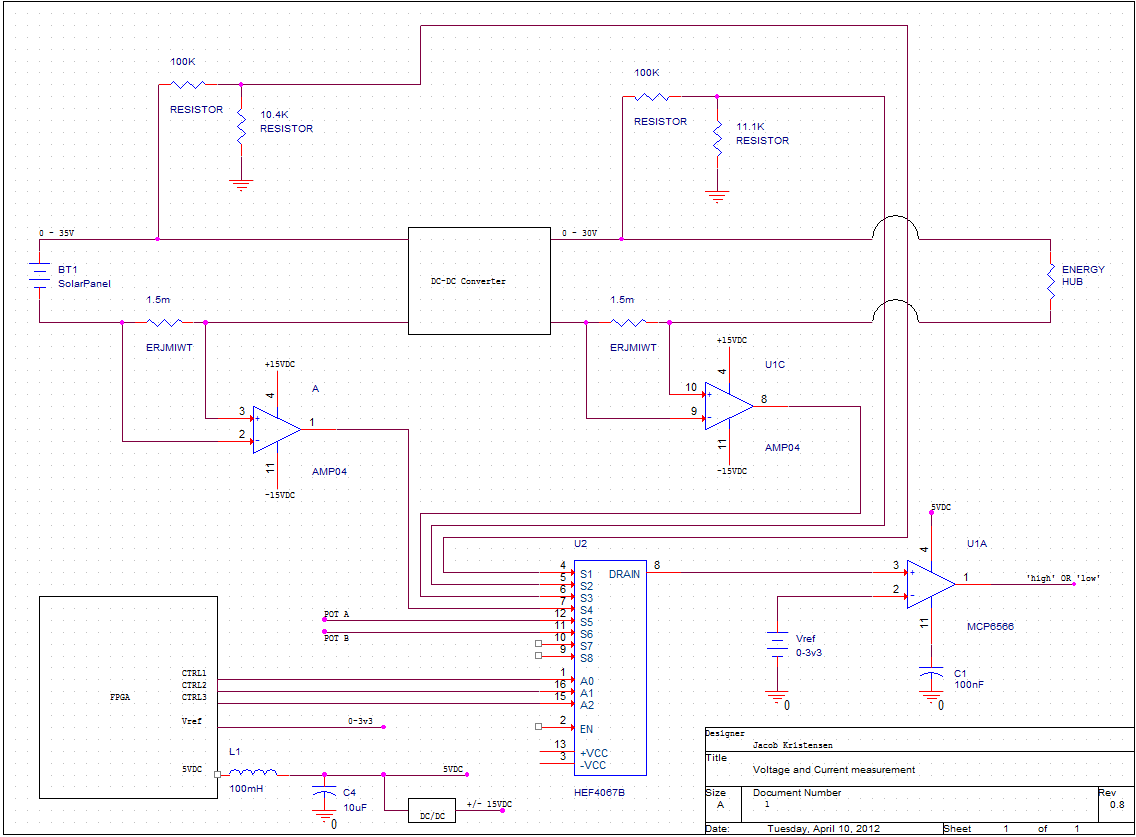
\includegraphics[width=20cm]{./img/vc_measure_schematic}
\caption{}
\label{fig:vc_measure_schematic}
\end{figure}
\end{landscape}

A schematic of the voltage/current measurement hardware is made, which is shown in figure \ref{fig:vc_measure_schematic}.\\
Leftmost a battery is placed, symbol of the Photo Voltaic. The maximum output has bin set to 35V, which is higher than the datasheet documents, but this is just to be sure. A PWM signal is used to compare the voltage, and not a R-ladder, which makes the steps smaller, and the measurement more precise. At the center the DC/DC converter is placed as a square. To the right a resistor is placed, symbol of the load (Energy Hub).\\
The voltage and the current has to be measured both before and after the DC/DC conversion. This gives two almost identical circuits on both sides of the DC/DC converter.\\
On top two voltage dividers is placed, to divide the voltage down to 3v3, which is the maximum input the FPGA can measure. A high input impedance of 100K ohm will ensure less loss in the circuit. \\
The equations to find the resistor values for the voltage dividers:\\
\begin{equation}
V_o=\frac{R_2}{R_1+R_2}*V_i
\end{equation}
\begin{equation}
3.3V=\frac{R_2}{100,000R+R_2}*35V
\end{equation}
\begin{center}
$R_2=10.4K ohm$
\end{center}

and now after the DC/DC, where the voltage must be at maximum 33VDC.
\begin{equation}
3.3V=\frac{R_2}{100,000R+R_2}*33V
\end{equation}
\begin{center}
$R_2=11.1K ohm$
\end{center}



Below the voltage dividers, two instrumental amplifiers (AMP04) are placed. They measure the voltage drop over a ERJMIWT (Power current measurement resistor), with an resistance of 1.5m ohm, which is very small, ensures as less loss in power as possible. These resistors are built for the purpose. \\
Also the instrumental amplifiers are optimized for measurements. They have a very low power consumption, they are very sensitive and does not get easily disturbed by interference from the surroundings, which makes them great for the purpose of measuring devices. \\
Both the outputs from the voltage dividers and from the amplifiers are sent to a multiplexer, which also receives the inputs from the pot-meters, measuring the position of the two motors turning the solar panel. They will be discussed later. The multiplexed signals will then be sent to a comperator (MCP6566), which receives a PWM reference input from the FPGA board. Then the FPGA can measure both current and voltage of input and output of the DC/DC converter. The multiplexer needs 3 signals to be controlled. \\
The instrumental amplifiers needs -+15VDC supply, which can be obtained by converting 5VDC into +-15VDC. This can be done by a converter from xppower.com. The 5VDC supply is placed on the FPGA board. This source can be very unstable, so in order to make it more stable, an LC circuit is placed at this output. This LC circuit consists of an inductor (L) and a capacitor(C). \\
To minimize the effect of fast-edges, and to decouple any track inductance, a de-coupling capacitor is added to the supply of the comparator. The capacitor should be placed as close to the amplifier as possible. Even though this will not be a big PCB, and thereby the track inductance wont be that big, it will not harm to place a 100mF capacitor at the supply. 


\paragraph{verification of requirements}\mbox{}\\

